% =====================================================================
% articulo.tex — Examen Parcial de Inteligencia Artificial II (CBS06 2026-2)
% Tema 7: Agentes adversarios duales para detección sin etiquetas.
% Clase apa7 (APA 7.ª ed.), modo revista "jou"; bibliografía biblatex-apa + biber.
% Compilar: pdflatex -> biber -> pdflatex -> pdflatex  (Overleaf lo hace solo).
% =====================================================================
\documentclass[jou,a4paper,floatsintext,donotrepeattitle]{apa7}

% ---------- Idioma y codificación -------------------------------------
\usepackage[T1]{fontenc}
\usepackage[utf8]{inputenc}
\usepackage[spanish,es-tabla,es-nodecimaldot,es-noshorthands]{babel}
\usepackage{csquotes}

% ---------- Matemáticas, tablas y figuras ------------------------------
\usepackage{amsmath,amssymb}
\usepackage{graphicx}
\usepackage{booktabs}
\usepackage{array}
\usepackage{tabularx}
\usepackage{multirow}

% ---------- Bibliografía APA 7 -----------------------------------------
\usepackage[style=apa,backend=biber]{biblatex}
\addbibresource{referencias.bib}

% ---------- Hipervínculos (cargar al final) ----------------------------
\usepackage{hyperref}
\hypersetup{colorlinks=true,linkcolor=black,citecolor=black,urlcolor=blue}

% ---------- Comandos auxiliares ----------------------------------------
\newcommand{\pend}[1]{\textbf{[DATO PENDIENTE: #1]}}   % marca de dato por completar
\newcommand{\vect}[1]{\mathbf{#1}}

% =====================================================================
%  PORTADA (datos del autor)
% =====================================================================
\title{Agentes adversarios duales LSTM--GAN para la detección no supervisada de comportamientos maliciosos en registros de servidores universitarios}
\shorttitle{Agentes adversarios duales para detección sin etiquetas}

% >>> COMPLETAR: nombre completo, código y filiación institucional <<<
\author{Arturo Ruiz Tarazona}
\affiliation{Facultad de Ingeniería Eléctrica y Electrónica (FIEE){,} Escuela Profesional de Ingeniería de Ciberseguridad\\
Universidad Nacional de Ingeniería (UNI){,} Lima{,} Perú\\
Curso de Inteligencia Artificial II (CBS06){,} semestre 2026-2}
\leftheader{Ruiz}

\abstract{Los registros (\textit{logs}) de servidores universitarios crecen a un ritmo que impide su revisión manual y carecen de etiquetas que permitan entrenar detectores supervisados. Este estudio evalúa si un modelo de agentes adversarios duales de reconstrucción latente, un autocodificador LSTM y un discriminador secuencial que compiten en un juego \textit{minimax} (LSTM--GAN), mejora la detección de comportamientos maliciosos frente a Isolation Forest, técnica no supervisada de referencia. Se empleó un diseño cuasi-experimental con medida pre-prueba/post-prueba sobre datos reales crudos: 3\,217\,544 eventos de PostgreSQL, GitLab y un ERP en Odoo, agrupados en 53\,416 ventanas de cinco minutos mediante Drain3 y Word2Vec. Los modelos se entrenaron sin etiquetas y se evaluaron con etiquetas débiles derivadas de reglas de seguridad, con partición cronológica y diez semillas por subconjunto (30 pares). El LSTM--GAN incrementó el puntaje F1 de 25.06\,\% a 32.26\,\% ($p < .001$, $r = .85$) y redujo la tasa de falsos positivos de 6.27\,\% a 2.88\,\% ($p = .002$, $r = .58$), sin diferencia significativa en el área bajo la curva ROC (86.52\,\% frente a 85.68\,\%; $p = .529$). El análisis de ablación mostró que el autocodificador sin componente adversarial alcanza un desempeño igual o superior y más estable. Se concluye que la reconstrucción temporal de series semánticas es eficaz para reducir falsas alarmas sin datos etiquetados, mientras que la contribución del discriminador debe justificarse empíricamente en cada entorno.}

\keywords{detección de anomalías, registros del sistema, autocodificador LSTM, red generativa adversarial, aprendizaje no supervisado, ciberseguridad}

\begin{document}
\def\keywordname{Palabras clave}\def\notelabel{Nota}
\maketitle

% =====================================================================
\section*{Ideas destacadas}
% =====================================================================
\begin{itemize}
  \item Un autocodificador LSTM con discriminador adversarial (LSTM--GAN) detecta inyecciones SQL y escaneos web en registros universitarios reales sin usar etiquetas.
  \item Frente a Isolation Forest, el LSTM--GAN eleva el F1 en 7.2 puntos y reduce las falsas alarmas en un 54\,\%, con significancia estadística en 30 pares.
  \item El componente adversarial no supera al autocodificador LSTM aislado, que obtiene la mayor capacidad discriminante (AUC de 89.04\,\%).
\end{itemize}

% =====================================================================
\section{1. Introducción}
% =====================================================================
Los sistemas informáticos registran de forma continua su actividad en archivos de \textit{logs}, que constituyen la principal fuente de evidencia para detectar fallos, usos indebidos e intrusiones. El volumen de estos registros en infraestructuras modernas hace inviable su inspección manual, y las reglas o firmas escritas a mano solo reconocen escenarios previstos de antemano, por lo que se requieren técnicas que aprendan automáticamente el comportamiento normal y señalen sus desviaciones \parencite{landauer2023}. En una universidad, un mismo conjunto de servidores aloja bases de datos académicas y administrativas, plataformas de control de versiones y aplicaciones de gestión expuestas a Internet, de modo que una intrusión en cualquiera de ellos compromete información sensible y la continuidad de los servicios.

La variable dependiente de este estudio es la \textit{detección de comportamientos maliciosos}, cuya problemática presenta tres rasgos. Primero, las anomalías son raras y no se conocen de antemano, por lo que rara vez existen etiquetas para entrenar clasificadores supervisados; obtenerlas a escala industrial es costoso y debe repetirse cuando cambia el comportamiento normal \parencite{albert2025}. Segundo, los métodos no supervisados tienden a producir un número elevado de falsos positivos, lo que satura a los operadores y reduce la confianza en las alertas \parencite{zamanzadeh2024}. Tercero, buena parte de los resultados publicados se obtienen sobre unos pocos conjuntos de referencia previamente etiquetados (HDFS, BGL, Thunderbird, OpenStack), con supuestos optimistas como entrenar solo con datos normales o ajustar umbrales sobre el propio conjunto de prueba \parencite{albert2025,landauer2023}.

Las arquitecturas basadas en reconstrucción ofrecen una alternativa sin etiquetas: un autocodificador aprende a reconstruir el comportamiento normal y las entradas que no logra reconstruir se consideran anómalas \parencite{zamanzadeh2024}. Su combinación con redes generativas adversariales (GAN), en las que un discriminador obliga al codificador a producir representaciones latentes más fieles, ha mostrado mejoras en series temporales industriales y de Internet de las cosas \parencite{gong2023,qian2025}. Sin embargo, \textbf{el vacío} que aborda este trabajo es la ausencia de evidencia sobre el desempeño de estos agentes adversarios duales en registros \emph{crudos y heterogéneos} de infraestructura universitaria real, sin etiquetas, con partición cronológica y comparados estadísticamente con una técnica tradicional.

El \textbf{propósito} del estudio es evaluar en qué medida un modelo LSTM--GAN de reconstrucción latente mejora la detección de comportamientos maliciosos sin etiquetas en registros de servidores universitarios. Los \textbf{objetivos específicos} son: (OE1) determinar su efecto sobre la exactitud de la detección (F1); (OE2) determinar su efecto sobre la tasa de falsas alarmas (FPR); y (OE3) determinar su efecto sobre la capacidad discriminante (AUC-ROC), en todos los casos frente a Isolation Forest. En coherencia, se plantea la hipótesis general de que el modelo LSTM--GAN mejora significativamente la detección y las hipótesis específicas H1 (aumenta el F1), H2 (reduce la FPR) y H3 (aumenta el AUC). La \textbf{motivación} es práctica: los equipos de seguridad universitarios disponen de abundantes registros pero no de analistas para etiquetarlos. La \textbf{importancia} radica en aportar un experimento reproducible con datos reales, que cuantifica el efecto del modelo y de su componente adversarial mediante ablación. El \textbf{aporte} incluye además una representación de ventanas de cinco minutos como series semánticas que corrige la debilidad de la reconstrucción secuencial ante ráfagas de ataque repetitivas.

% =====================================================================
\section{2. Revisión de la literatura}
% =====================================================================
\textcite{landauer2023} revisaron sistemáticamente 62 enfoques de aprendizaje profundo para detectar anomalías en \textit{logs}. Identificaron que las redes recurrentes son las más usadas, que los autocodificadores y las GAN son las opciones naturales para el aprendizaje no supervisado y que casi todas las evaluaciones dependen de cuatro conjuntos de datos con anomalías de tipo secuencial. Advirtieron, además, que heurísticas simples alcanzan resultados competitivos en HDFS. Por ello recomendaron evaluar con datos más diversos que incluyan artefactos de ciberataques y no solo fallos.

\textcite{albert2025} demostró que los métodos semi-supervisados del estado del arte colapsan cuando el conjunto de entrenamiento contiene anomalías mezcladas, condición habitual en datos industriales sin depurar. También mostró que la división cronológica, frente a la aleatoria, reduce drásticamente el F1 reportado: en BGL, de 92.7\,\% a 42.6\,\% con DeepLog. Esto evidencia que la literatura sobreestima el desempeño esperable en producción.

En el plano arquitectónico, \textcite{gong2023} propusieron un autocodificador recurrente asistido por una GAN. En él, el discriminador distingue la codificación latente de la entrada de la recodificación de su reconstrucción, y el conjunto superó a métodos clásicos en datos industriales. \textcite{qian2025} integraron autocodificadores y GAN en RGAnomaly y combinaron la pérdida de reconstrucción con la de discriminación en una puntuación única de anomalía. Ambos trabajos se validaron con series de sensores, no con registros de texto.

\textcite{nasirzadeh2025} alcanzaron un F1 medio de 99.61\,\% en siete conjuntos de \textit{logs} de sistemas operativos, pero con un enfoque supervisado que requiere etiquetas. En síntesis, la literatura evidencia el potencial de los modelos adversariales de reconstrucción, pero no responde si aportan valor frente a técnicas tradicionales en registros universitarios reales, sin etiquetas y evaluados con rigor cronológico. Ese es el vacío que aborda este estudio.

% =====================================================================
\section{3. Metodología}
% =====================================================================
\subsection{3.1. Enfoque, tipo y diseño}
El estudio es cuantitativo, de tipo aplicado y de nivel explicativo. Se adoptó un diseño cuasi-experimental de comparación con medida pre-prueba/post-prueba sobre las mismas unidades. La pre-prueba corresponde al desempeño de la técnica tradicional (Isolation Forest), el estímulo es la implementación del modelo LSTM--GAN y la post-prueba es el desempeño de este último sobre idénticas ventanas de evaluación. Se eligió este diseño porque permite atribuir las diferencias al modelo y no a la muestra, y porque contrastar un modelo propuesto con líneas de base sobre los mismos datos es la práctica habitual del área \parencite{landauer2023,nasirzadeh2025}. Se añadió un tercer tratamiento de ablación (LSTM-AE sin discriminador) para aislar la contribución del componente adversarial.

\subsection{3.2. Descripción del conjunto de datos real}
Se utilizaron registros \emph{crudos} del repositorio institucional \textit{uni-logs}, publicado por el docente (\url{https://uni-logs.us-mia-1.linodeobjects.com/list.html}). Se analizaron tres de sus cuatro subconjuntos, que se describen en la Tabla~\ref{tab:datos}:

\begin{itemize}
  \item \texttt{logdb}: servidor PostgreSQL 12.
  \item \texttt{loggit}: plataforma GitLab, con registros de acceso de nginx, \texttt{sshd} y \texttt{gitlab-shell}.
  \item \texttt{logsapp}: ERP CubicERP basado en Odoo, con registros del servidor principal, del servidor \textit{gevent} y de gunicorn.
\end{itemize}

Se excluyeron los registros de instalación del sistema operativo (\texttt{dpkg}, \texttt{apt}, \texttt{bootstrap}) por no reflejar la operación del servicio. La población la constituye la totalidad de eventos registrados; la muestra, obtenida por conveniencia, comprende 3\,217\,544 eventos agrupados en 53\,416 ventanas.

% >>> Tabla 1: caracterización de los datos (valores de out/tabla_dataset.csv)
\begin{table*}[t]
\caption{Caracterización de los subconjuntos de registros crudos analizados}
\label{tab:datos}
\centering
\footnotesize\setlength{\tabcolsep}{2.5pt}
\begin{tabular}{@{}llrrrlrr@{}}
\toprule
Subconjunto & Fuente & Eventos & Plantillas & Ventanas & Periodo (UTC) & Ent./Val./Prueba & Maliciosas (E/V/P) \\
\midrule
\texttt{logdb}   & PostgreSQL 12   & 267\,896   & 186 & 5\,719  & 01/03/2026 -- 12/05/2026 & 3\,431 / 1\,144 / 1\,144 & 2 / 1 / 90 \\
\texttt{loggit}  & GitLab          & 56\,135    & 121 & 3\,398  & 30/10/2025 -- 12/05/2026 & 2\,038 / 680 / 680      & 38 / 28 / 21 \\
\texttt{logsapp} & CubicERP (Odoo) & 2\,893\,513 & 361 & 44\,299 & 20/11/2025 -- 12/05/2026 & 26\,579 / 8\,860 / 8\,860 & 24 / 2 / 8 \\
\midrule
Total            &                 & 3\,217\,544 & 668 & 53\,416 &                          & 32\,048 / 10\,684 / 10\,684 & 64 / 31 / 119 \\
\bottomrule
\end{tabular}
\figurenote{Ventanas de cinco minutos con al menos un evento. Las ventanas maliciosas corresponden a etiquetas débiles (Tabla~\ref{tab:reglas}), usadas solo para evaluar. E = entrenamiento; V = validación; P = prueba.}
\end{table*}

\subsection{3.3. Técnicas e instrumentos de recolección}
La técnica fue el análisis documental de registros digitales. Los instrumentos fueron tres:

\begin{itemize}
  \item El analizador de plantillas Drain3, que separa la parte constante de cada mensaje de sus parámetros variables mediante un árbol de profundidad fija \parencite{nasirzadeh2025,zhao2025}.
  \item Una ficha de reglas de seguridad para generar etiquetas débiles de referencia (Tabla~\ref{tab:reglas}; Apéndice~C).
  \item Los guiones reproducibles en Python (PyTorch, scikit-learn, gensim), que registran cada corrida.
\end{itemize}

El etiquetado por reglas o términos indicativos tiene precedente en \textcite{nasirzadeh2025}. Es pertinente aquí porque los registros no incluyen etiquetas. Las etiquetas \emph{no} se usan para entrenar ningún modelo, solo para evaluarlos.

% >>> Tabla 2: instrumento de etiquetado débil
\begin{table}[t]
\caption{Reglas de seguridad para el etiquetado débil por ventana}
\label{tab:reglas}
\small
\begin{tabularx}{\columnwidth}{@{}lX@{}}
\toprule
Subconjunto & Una ventana se etiqueta como maliciosa si \ldots \\
\midrule
\texttt{logdb} & contiene $\geq 1$ firma de inyección SQL (\texttt{sleep(}, \texttt{XOR(}, \texttt{OR n=n}, \texttt{UNION SELECT}) o $\geq 3$ fallos de sondeo (base de datos o rol inexistente, autenticación fallida). \\
\texttt{loggit} & contiene $\geq 1$ URL con carga de ataque (SQLi/XSS, \textit{path traversal}, \texttt{.php}, \texttt{wp-*}, \texttt{.env}), $\geq 1$ agente escáner, $\geq 3$ fallos SSH o $\geq 10$ respuestas HTTP 4xx. \\
\texttt{logsapp} & contiene $\geq 1$ URL con carga de ataque o $\geq 10$ respuestas HTTP 4xx. \\
\bottomrule
\end{tabularx}
\figurenote{Se excluye el código 499 (cierre de conexión por el cliente) porque no indica una petición errónea.}
\end{table}

\subsection{3.4. Procedimiento experimental}
El protocolo se ejecutó en tres fases automatizadas.

\begin{itemize}
  \item \textbf{Fase de preparación.} Se leyeron los registros, se convirtieron todas las marcas de tiempo a UTC y se unieron las líneas de continuación de trazas y sentencias SQL. Las líneas de acceso web se codificaron como \textit{método–primer segmento de ruta–extensión–estado HTTP–familia de agente}, para que Drain3 conservara la señal de ataque. Después, Drain3 se aplicó en línea, en orden cronológico, y los eventos se agruparon en ventanas fijas de cinco minutos, estrategia recomendada cuando no existen identificadores de sesión \parencite{landauer2023}.
  \item \textbf{Partición.} Cada subconjunto se dividió cronológicamente en 60\,\% para entrenamiento, 20\,\% para validación y 20\,\% para prueba. Así se evita la fuga de información futura señalada por \textcite{albert2025}. El conjunto de entrenamiento \emph{no} se depuró, por lo que contiene 64 ventanas maliciosas; el escenario es, por tanto, genuinamente no supervisado.
  \item \textbf{Pre-prueba y estímulo.} Isolation Forest, LSTM-AE y LSTM--GAN se entrenaron sobre las mismas ventanas, con diez semillas aleatorias por subconjunto.
  \item \textbf{Post-prueba.} El umbral de decisión $\rho$ de cada modelo se fijó en el percentil 95 de sus puntuaciones de validación, sin intervención del tramo de prueba \parencite{albert2025,qian2025}, y se calcularon los indicadores sobre el tramo de prueba.
\end{itemize}

\subsection{3.5. Indicadores y análisis estadístico}
La exactitud se midió con el puntaje F1, la precisión y la exhaustividad; las falsas alarmas, con la FPR y la especificidad; y la capacidad discriminante, con el AUC-ROC y el coeficiente de correlación de Matthews (MCC) \parencite{almodovar2024,zhang2025,zamanzadeh2024}:
\begin{equation}
F1 = \frac{2PR}{P+R}, \qquad FPR = \frac{FP}{FP+TN}.
\label{eq:metricas}
\end{equation}
El AUC-ROC es independiente del umbral, lo que lo hace adecuado para comparar puntuaciones continuas \parencite{gorokhov2023}. Para cada indicador se calcularon la media, la desviación estándar, la diferencia absoluta $\Delta = \text{post} - \text{pre}$ y la variación relativa.

La prueba de Shapiro–Wilk rechazó la normalidad de las diferencias en F1, FPR y AUC ($p < .05$). Por ello, las hipótesis se contrastaron con la prueba de rangos con signo de Wilcoxon para muestras relacionadas, con $\alpha = .05$, sobre 30 pares (10 semillas $\times$ 3 subconjuntos) y por subconjunto (10 pares), con tamaño del efecto $r = Z/\sqrt{n}$. Como análisis complementario, se estimó mediante \textit{bootstrap} (2\,000 remuestreos) el intervalo de confianza al 95\,\% de la diferencia de AUC a nivel de ventana.

\subsection{3.6. Comparación con metodologías similares}
El preprocesamiento sigue la cadena análisis de plantillas, representación semántica y agrupación por ventanas de \textcite{zhao2025} y \textcite{zhang2025}, que también emplean Drain y Word2Vec. El criterio de anomalía por error de reconstrucción coincide con \textcite{aslam2024} y \textcite{gong2023}. La puntuación que combina reconstrucción y discriminación procede de \textcite{qian2025}.

El estudio se diferencia de esos trabajos en tres aspectos: usa datos crudos sin depurar en lugar de conjuntos de referencia etiquetados, aplica una partición estrictamente cronológica y somete el resultado a pruebas de significancia y a ablación, elementos poco frecuentes en la literatura revisada \parencite{landauer2023}.

% =====================================================================
\section{4. Desarrollo}
% =====================================================================
Los modelos se organizan jerárquicamente en tres niveles de complejidad creciente. El primero es Isolation Forest, puntual y sin contexto temporal. El segundo es el LSTM-AE, que añade contexto temporal y reconstrucción. El tercero es el LSTM--GAN, que añade el discriminador adversarial. La Figura~\ref{fig:arquitectura} resume el flujo.

% >>> Figura 1: diagrama de la arquitectura (dibujado con TikZ)
\begin{figure}[t]
\caption{Arquitectura del modelo LSTM--GAN de agentes adversarios duales}
\label{fig:arquitectura}
\centering
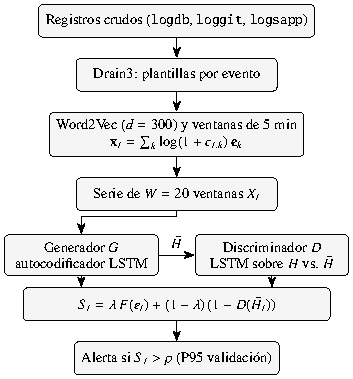
\includegraphics[width=\columnwidth]{figs/fig0_arquitectura.pdf}
% (Diagrama precompilado desde fig0.tex con TikZ para acelerar la compilación)
\figurenote{Elaboración propia. $F(\cdot)$ es la función de distribución empírica del error de reconstrucción en validación.}
\end{figure}

\subsection{4.1. Representación semántica de las ventanas}
Cada plantilla $k$ se representa mediante el promedio normalizado $\vect{e}_k \in \mathbb{R}^{300}$ de los vectores Word2Vec (\textit{skip-gram}) de sus términos, entrenados sobre el vocabulario de plantillas sin usar etiquetas \parencite{zhao2025}. Cada ventana $t$ con conteos $c_{t,k}$ se representa como
\begin{equation}
\vect{x}_t = \sum_{k} \log\!\left(1 + c_{t,k}\right)\vect{e}_k,
\label{eq:ventana}
\end{equation}
estandarizado con la media y la desviación del tramo de entrenamiento. La entrada del modelo es la serie $X_t = (\vect{x}_{t-W+1}, \ldots, \vect{x}_t)$ con $W = 20$ (100 minutos) y paso 1, de modo que cada ventana recibe una puntuación propia.

Esta decisión corrige un problema detectado en pruebas preliminares. Al modelar secuencias de \emph{eventos}, las ráfagas de ataque, compuestas por cientos de peticiones idénticas, resultaban trivialmente reconstruibles y obtenían puntuaciones bajas.

\subsection{4.2. Línea de base: Isolation Forest}
Isolation Forest aísla observaciones mediante particiones aleatorias recursivas: las anomalías requieren menos particiones para quedar aisladas. Es una referencia no supervisada habitual en este dominio \parencite{landauer2023,nasirzadeh2025}. Se usaron 200 árboles sobre el vector $\log(1+c_{t,k})$ de cada ventana, y la puntuación de anomalía es la puntuación de aislamiento con signo invertido.

\subsection{4.3. Generador: autocodificador LSTM}
El codificador LSTM recorre la serie y la resume en el estado oculto final $\vect{z}_t = \vect{h}_W \in \mathbb{R}^{128}$:
\begin{equation}
\vect{h}_i = \mathrm{LSTM}_{enc}(\vect{x}_i, \vect{h}_{i-1}).
\end{equation}
El decodificador recibe $\vect{z}_t$ en cada paso y reconstruye la serie, $\hat{\vect{x}}_i = W_o\,\mathrm{LSTM}_{dec}(\vect{z}_t, \vect{s}_{i-1}) + \vect{b}_o$. La pérdida de reconstrucción es el error cuadrático medio sobre las posiciones válidas $m_i$:
\begin{equation}
\mathcal{L}_{rec} = \frac{1}{\sum_i m_i}\sum_{i=1}^{W} m_i \lVert \vect{x}_i - \hat{\vect{x}}_i \rVert_2^2 .
\label{eq:rec}
\end{equation}

\subsection{4.4. Discriminador adversario secuencial}
Siguiendo a \textcite{gong2023}, el discriminador $D$ es una LSTM de 64 unidades con salida sigmoide. Recibe la secuencia de estados ocultos $H = \vect{h}_{1:W}$ de la entrada real y la secuencia $\tilde H = \mathrm{LSTM}_{enc}(\hat X)$ obtenida al recodificar la reconstrucción, y aprende a distinguirlas. El entrenamiento alterna dos pasos:
\begin{gather}
\mathcal{L}_{D} = -\left[\log D(H) + \log\!\left(1 - D(\tilde H)\right)\right], \label{eq:ld}\\
\mathcal{L}_{G} = \alpha\,\mathcal{L}_{rec} + (1-\alpha)\left[-\log D(\tilde H)\right], \label{eq:lg}
\end{gather}
con $\alpha = 0.8$. La ecuación~\eqref{eq:lg} obliga al generador a producir reconstrucciones cuya codificación latente sea indistinguible de la real.

\subsection{4.5. Puntuación dual y decisión}
Para cada ventana se combinan el error de reconstrucción de su última posición, $e_t = \lVert \vect{x}_t - \hat{\vect{x}}_t \rVert_2^2$, y el rechazo del discriminador \parencite{qian2025}:
\begin{equation}
S_t = \lambda\,F_{val}(e_t) + (1-\lambda)\left(1 - D(\tilde H_t)\right),
\label{eq:score}
\end{equation}
donde $F_{val}$ es la función de distribución empírica del error en validación, que lleva ambos términos a la escala $[0,1]$, y $\lambda = 0.7$. La ventana se clasifica como maliciosa si $S_t > \rho$. El LSTM-AE de ablación usa $S_t = F_{val}(e_t)$ y se entrena solo con la ecuación~\eqref{eq:rec}. La Tabla~\ref{tab:hiper} resume la configuración.

% >>> Tabla 3: hiperparámetros
\begin{table}[t]
\caption{Configuración de los modelos}
\label{tab:hiper}
\small
\begin{tabularx}{\columnwidth}{@{}Xr@{}}
\toprule
Parámetro & Valor \\
\midrule
Dimensión Word2Vec / estado oculto LSTM & 300 / 128 \\
Ventanas por serie ($W$) / paso & 20 / 1 \\
Unidades del discriminador & 64 \\
$\alpha$ (peso de $\mathcal{L}_{rec}$) / $\lambda$ (peso en $S_t$) & 0.8 / 0.7 \\
Optimizador / tasa de aprendizaje & Adam / $10^{-3}$ \\
Tamaño de lote / máx.\ secuencias por época & 1\,024 / 8\,192 \\
Épocas máximas / paciencia (parada temprana) & 30 / 5 \\
Árboles de Isolation Forest & 200 \\
Umbral $\rho$ & P95 de validación \\
Semillas por subconjunto & 10 \\
\bottomrule
\end{tabularx}
\figurenote{El límite de 8\,192 secuencias por época solo afecta a \texttt{logsapp}.}
\end{table}

% =====================================================================
\section{5. Resultados}
% =====================================================================
\subsection{5.1. Desempeño por modelo y subconjunto}
La Tabla~\ref{tab:resultados} y la Figura~\ref{fig:indicadores} presentan los indicadores en el tramo de prueba. En el consolidado de los tres subconjuntos, el LSTM--GAN obtuvo F1 = 32.26\,\%, FPR = 2.88\,\% y AUC = 85.68\,\%. Isolation Forest obtuvo F1 = 25.06\,\%, FPR = 6.27\,\% y AUC = 86.52\,\%. Esto equivale a $\Delta$F1 = +7.19 puntos porcentuales (+28.7\,\%) y $\Delta$FPR = $-3.39$ puntos ($-54.0$\,\%). El LSTM-AE obtuvo F1 = 33.56\,\%, FPR = 3.28\,\% y AUC = 89.04\,\%.

Por subconjunto, el LSTM--GAN mejoró el F1 en \texttt{logdb} (+6.95), \texttt{loggit} (+13.60) y \texttt{logsapp} (+1.03). Redujo la FPR en \texttt{logdb} ($-1.39$) y, sobre todo, en \texttt{logsapp} ($-9.53$, de 12.49\,\% a 2.95\,\%). En \texttt{loggit}, en cambio, aumentó la FPR (+0.76) y redujo el AUC ($-8.94$).

El F1 de \texttt{logsapp} es bajo para todos los modelos ($< 3$\,\%) porque el tramo de prueba contiene solo 8 ventanas maliciosas entre 8\,860. Con un umbral en el percentil 95, cualquier modelo emite cientos de alertas por cada verdadero positivo.

% >>> Tabla 4: resultados (out/tabla_descriptiva.csv)
\begin{table*}[t]
\caption{Indicadores de detección en el tramo de prueba (media $\pm$ desviación estándar de 10 semillas)}
\label{tab:resultados}
\centering
\small
\begin{tabular}{@{}llrrrrrr@{}}
\toprule
Subconjunto & Modelo & F1 (\%) & Precisión (\%) & Exhaustividad (\%) & FPR (\%) & AUC (\%) & MCC \\
\midrule
\multirow{3}{*}{\texttt{logdb}}
 & Isolation Forest & 25.33 $\pm$ 1.96 & 26.86 & 24.00 & 5.57 $\pm$ 0.30 & 80.15 $\pm$ 1.40 & .19 \\
 & LSTM-AE          & 32.89 $\pm$ 1.44 & 37.70 & 29.22 & 4.16 $\pm$ 0.49 & 83.88 $\pm$ 1.63 & .28 \\
 & LSTM--GAN        & 32.28 $\pm$ 1.34 & 37.02 & 28.67 & 4.18 $\pm$ 0.42 & 81.67 $\pm$ 2.17 & .28 \\
\midrule
\multirow{3}{*}{\texttt{loggit}}
 & Isolation Forest & 49.03 $\pm$ 6.88 & 64.30 & 40.00 & 0.74 $\pm$ 0.35 & 94.44 $\pm$ 0.43 & .49 \\
 & LSTM-AE          & 65.00 $\pm$ 3.96 & 84.65 & 52.86 & 0.30 $\pm$ 0.00 & 86.70 $\pm$ 0.80 & .66 \\
 & LSTM--GAN        & 62.64 $\pm$ 7.61 & 63.71 & 65.24 & 1.50 $\pm$ 1.15 & 85.50 $\pm$ 1.18 & .62 \\
\midrule
\multirow{3}{*}{\texttt{logsapp}}
 & Isolation Forest & 0.82 $\pm$ 0.12 & 0.41 & 57.50 & 12.49 $\pm$ 1.40 & 84.97 $\pm$ 1.67 & .04 \\
 & LSTM-AE          & 2.81 $\pm$ 0.15 & 1.43 & 86.25 & 5.39 $\pm$ 0.49 & 96.54 $\pm$ 0.36 & .11 \\
 & LSTM--GAN        & 1.85 $\pm$ 1.09 & 0.96 & 33.75 & 2.95 $\pm$ 1.43 & 89.88 $\pm$ 7.51 & .05 \\
\midrule
\multirow{3}{*}{Consolidado}
 & Isolation Forest & 25.06 & 30.53 & 40.50 & 6.27 & 86.52 & .24 \\
 & LSTM-AE          & 33.56 & 41.26 & 56.11 & 3.28 & 89.04 & .35 \\
 & LSTM--GAN        & 32.26 & 33.90 & 42.55 & 2.88 & 85.68 & .32 \\
\bottomrule
\end{tabular}
\figurenote{Umbral $\rho$ en el percentil 95 de validación. FPR: menor es mejor.}
\end{table*}

% >>> Figura 2: out/figs/fig1_indicadores.png
\begin{figure*}[t]
\caption{F1, tasa de falsos positivos y AUC por modelo y subconjunto}
\label{fig:indicadores}
\centering
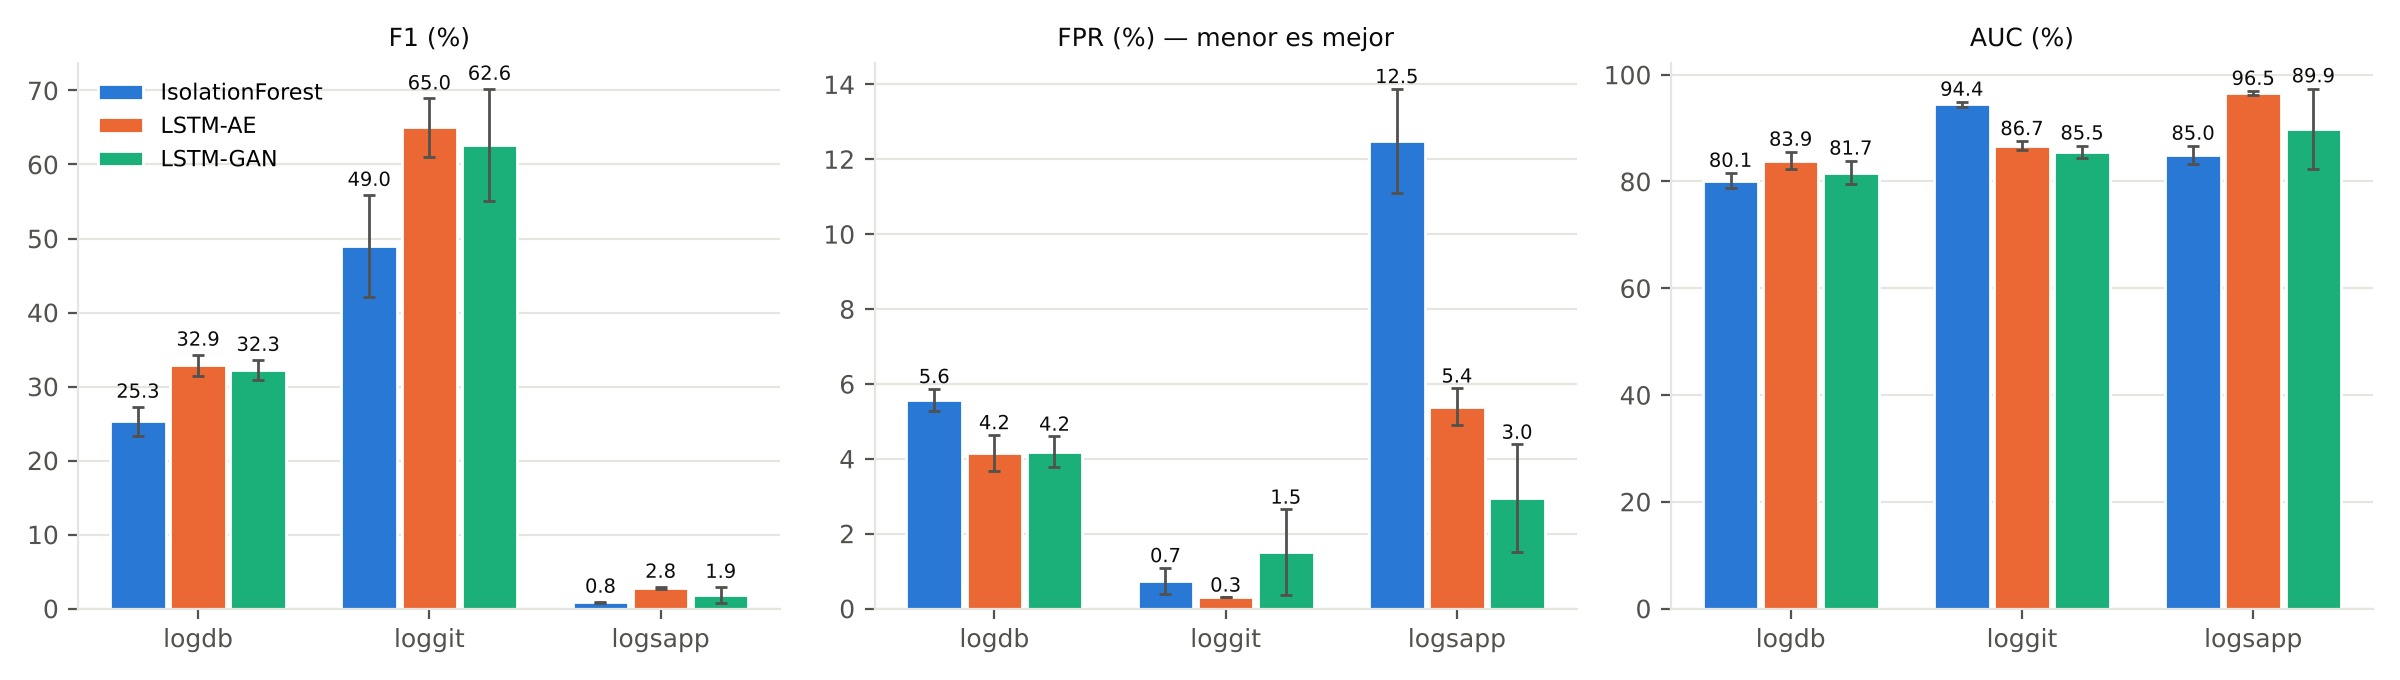
\includegraphics[width=\textwidth]{figs/fig1_indicadores.jpg}
\figurenote{Barras: media de 10 semillas; líneas de error: desviación estándar.}
\end{figure*}

\subsection{5.2. Contraste de hipótesis}
La Tabla~\ref{tab:hipotesis} muestra los contrastes de Wilcoxon. H1 se confirma: el LSTM--GAN aumentó el F1 de forma significativa en el consolidado y en los tres subconjuntos. H2 se confirma en el consolidado, en \texttt{logdb} y en \texttt{logsapp}, aunque en \texttt{loggit} la FPR aumentó significativamente. H3 no se confirma, porque la diferencia de AUC no fue significativa en el consolidado ($p = .529$) y fue desfavorable en \texttt{loggit}.

El \textit{bootstrap} a nivel de ventana confirma el patrón mixto del AUC:

\begin{itemize}
  \item \texttt{logdb}: diferencia de +1.71 puntos, IC~95\,\% [$-0.57$, 4.07].
  \item \texttt{loggit}: diferencia de $-8.87$ puntos, IC~95\,\% [$-19.85$, $-0.62$].
  \item \texttt{logsapp}: diferencia de +8.36 puntos, IC~95\,\% [2.21, 15.48].
\end{itemize}

Las curvas ROC se presentan en la Figura~\ref{fig:roc}.

% >>> Tabla 5: contraste de hipótesis (out/tabla_inferencial*.csv)
\begin{table}[t]
\caption{Contraste de hipótesis: LSTM--GAN frente a Isolation Forest (prueba de Wilcoxon)}
\label{tab:hipotesis}
\small
\begin{tabularx}{\columnwidth}{@{}lXrrr@{}}
\toprule
Hip. & Ámbito & $\bar{\Delta}$ & $p$ & $r$ \\
\midrule
H1 (F1)  & Consolidado ($n=30$) & +7.19 & $<.001$ & .85 \\
         & \texttt{logdb} / \texttt{loggit} / \texttt{logsapp} & + / + / + & .002 / .002 / .027 & \\
H2 (FPR) & Consolidado ($n=30$) & $-3.39$ & .002 & .58 \\
         & \texttt{logdb} / \texttt{loggit} / \texttt{logsapp} & $-$ / + / $-$ & .002 / .035 / .002 & \\
H3 (AUC) & Consolidado ($n=30$) & $-0.84$ & .529 & .12 \\
         & \texttt{logdb} / \texttt{loggit} / \texttt{logsapp} & + / $-$ / + & .106 / .002 / .160 & \\
\bottomrule
\end{tabularx}
\figurenote{$\bar{\Delta}$ = media de la diferencia LSTM--GAN menos Isolation Forest, en puntos porcentuales. Los signos por subconjunto indican la dirección del cambio; $n = 10$ pares en cada uno.}
\end{table}

% >>> Figura 3: out/figs/fig2_roc.png
\begin{figure*}[t]
\caption{Curvas ROC en el tramo de prueba (puntuaciones promediadas sobre 10 semillas)}
\label{fig:roc}
\centering
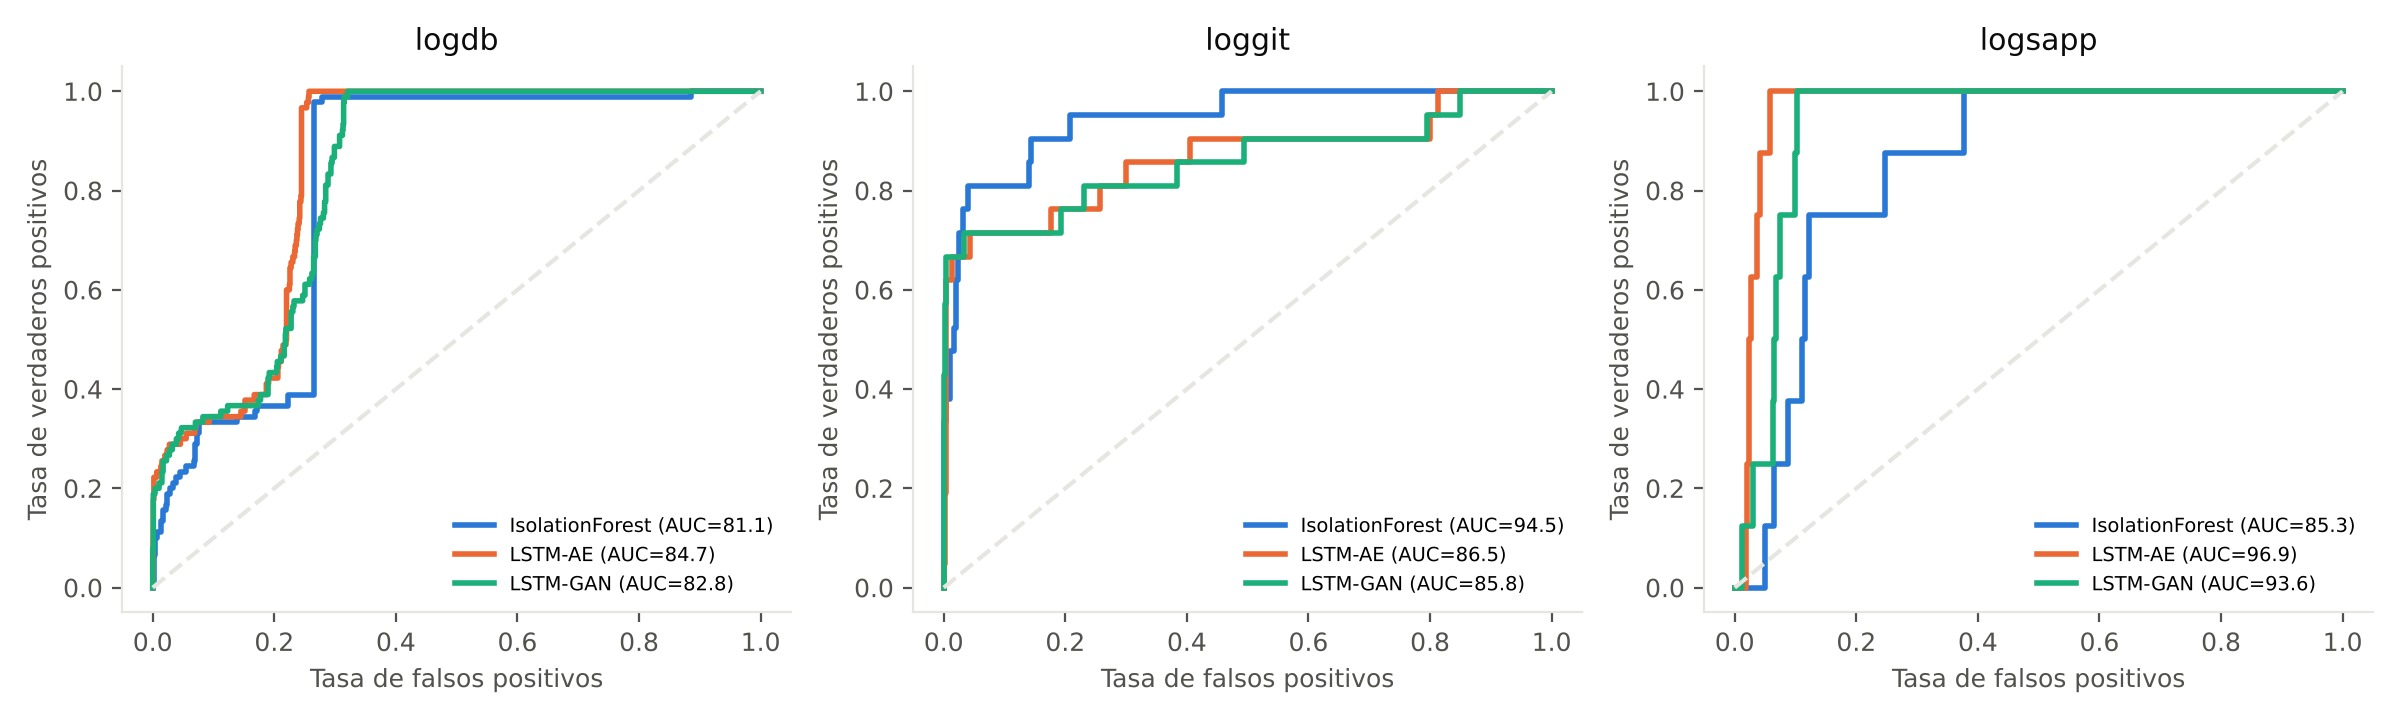
\includegraphics[width=\textwidth]{figs/fig2_roc.jpg}
\end{figure*}

\subsection{5.3. Análisis de ablación y sensibilidad}
Al retirar el discriminador (LSTM-AE), no hubo diferencias significativas en F1 ($p = .129$) ni en FPR ($p = .311$). El AUC, en cambio, mejoró en 3.36 puntos ($p < .001$, $r = .92$) y el MCC también fue mayor ($p = .002$). Además, el LSTM--GAN fue más inestable: en \texttt{logsapp}, la desviación de su AUC fue de 7.51 puntos frente a 0.36 del LSTM-AE.

Al elevar el umbral al percentil 99, el LSTM--GAN mantuvo un F1 de 33.68\,\% en \texttt{logdb}, con FPR = 1.69\,\%, mientras que Isolation Forest descendió a 19.96\,\%. En \texttt{loggit}, el LSTM--GAN obtuvo 44.39\,\% frente a 30.60\,\% de Isolation Forest. Su ventaja, por tanto, no depende de un umbral particular.

\subsection{5.4. Hallazgos cualitativos}
La Figura~\ref{fig:serie} muestra la puntuación $S_t$ en el tramo de prueba. El modelo detectó, sin etiquetas, campañas reales de ataque:

\begin{itemize}
  \item Inyecciones SQL ciegas basadas en tiempo (\texttt{sleep()}, \texttt{XOR}) contra PostgreSQL, el 1 y el 2 de mayo de 2026.
  \item Escaneos de \textit{webshells} \texttt{.php} y de \texttt{/wp-login.php} contra GitLab, servicio que no ejecuta PHP.
  \item Sondeos de archivos \texttt{.env} y de \texttt{cgi-bin} contra el ERP.
\end{itemize}

Hubo también un caso que el modelo no detectó: una enumeración lenta de bases de datos el 8 de mayo, con unos 630 intentos repartidos en cinco horas. Superó el umbral al inicio, pero el contexto de 100 minutos la absorbió como comportamiento habitual.

% >>> Figura 4: out/figs/fig3_serie_puntuacion.png
\begin{figure*}[t]
\caption{Puntuación $S_t$ del LSTM--GAN, umbral $\rho$ y ventanas maliciosas en el tramo de prueba}
\label{fig:serie}
\centering
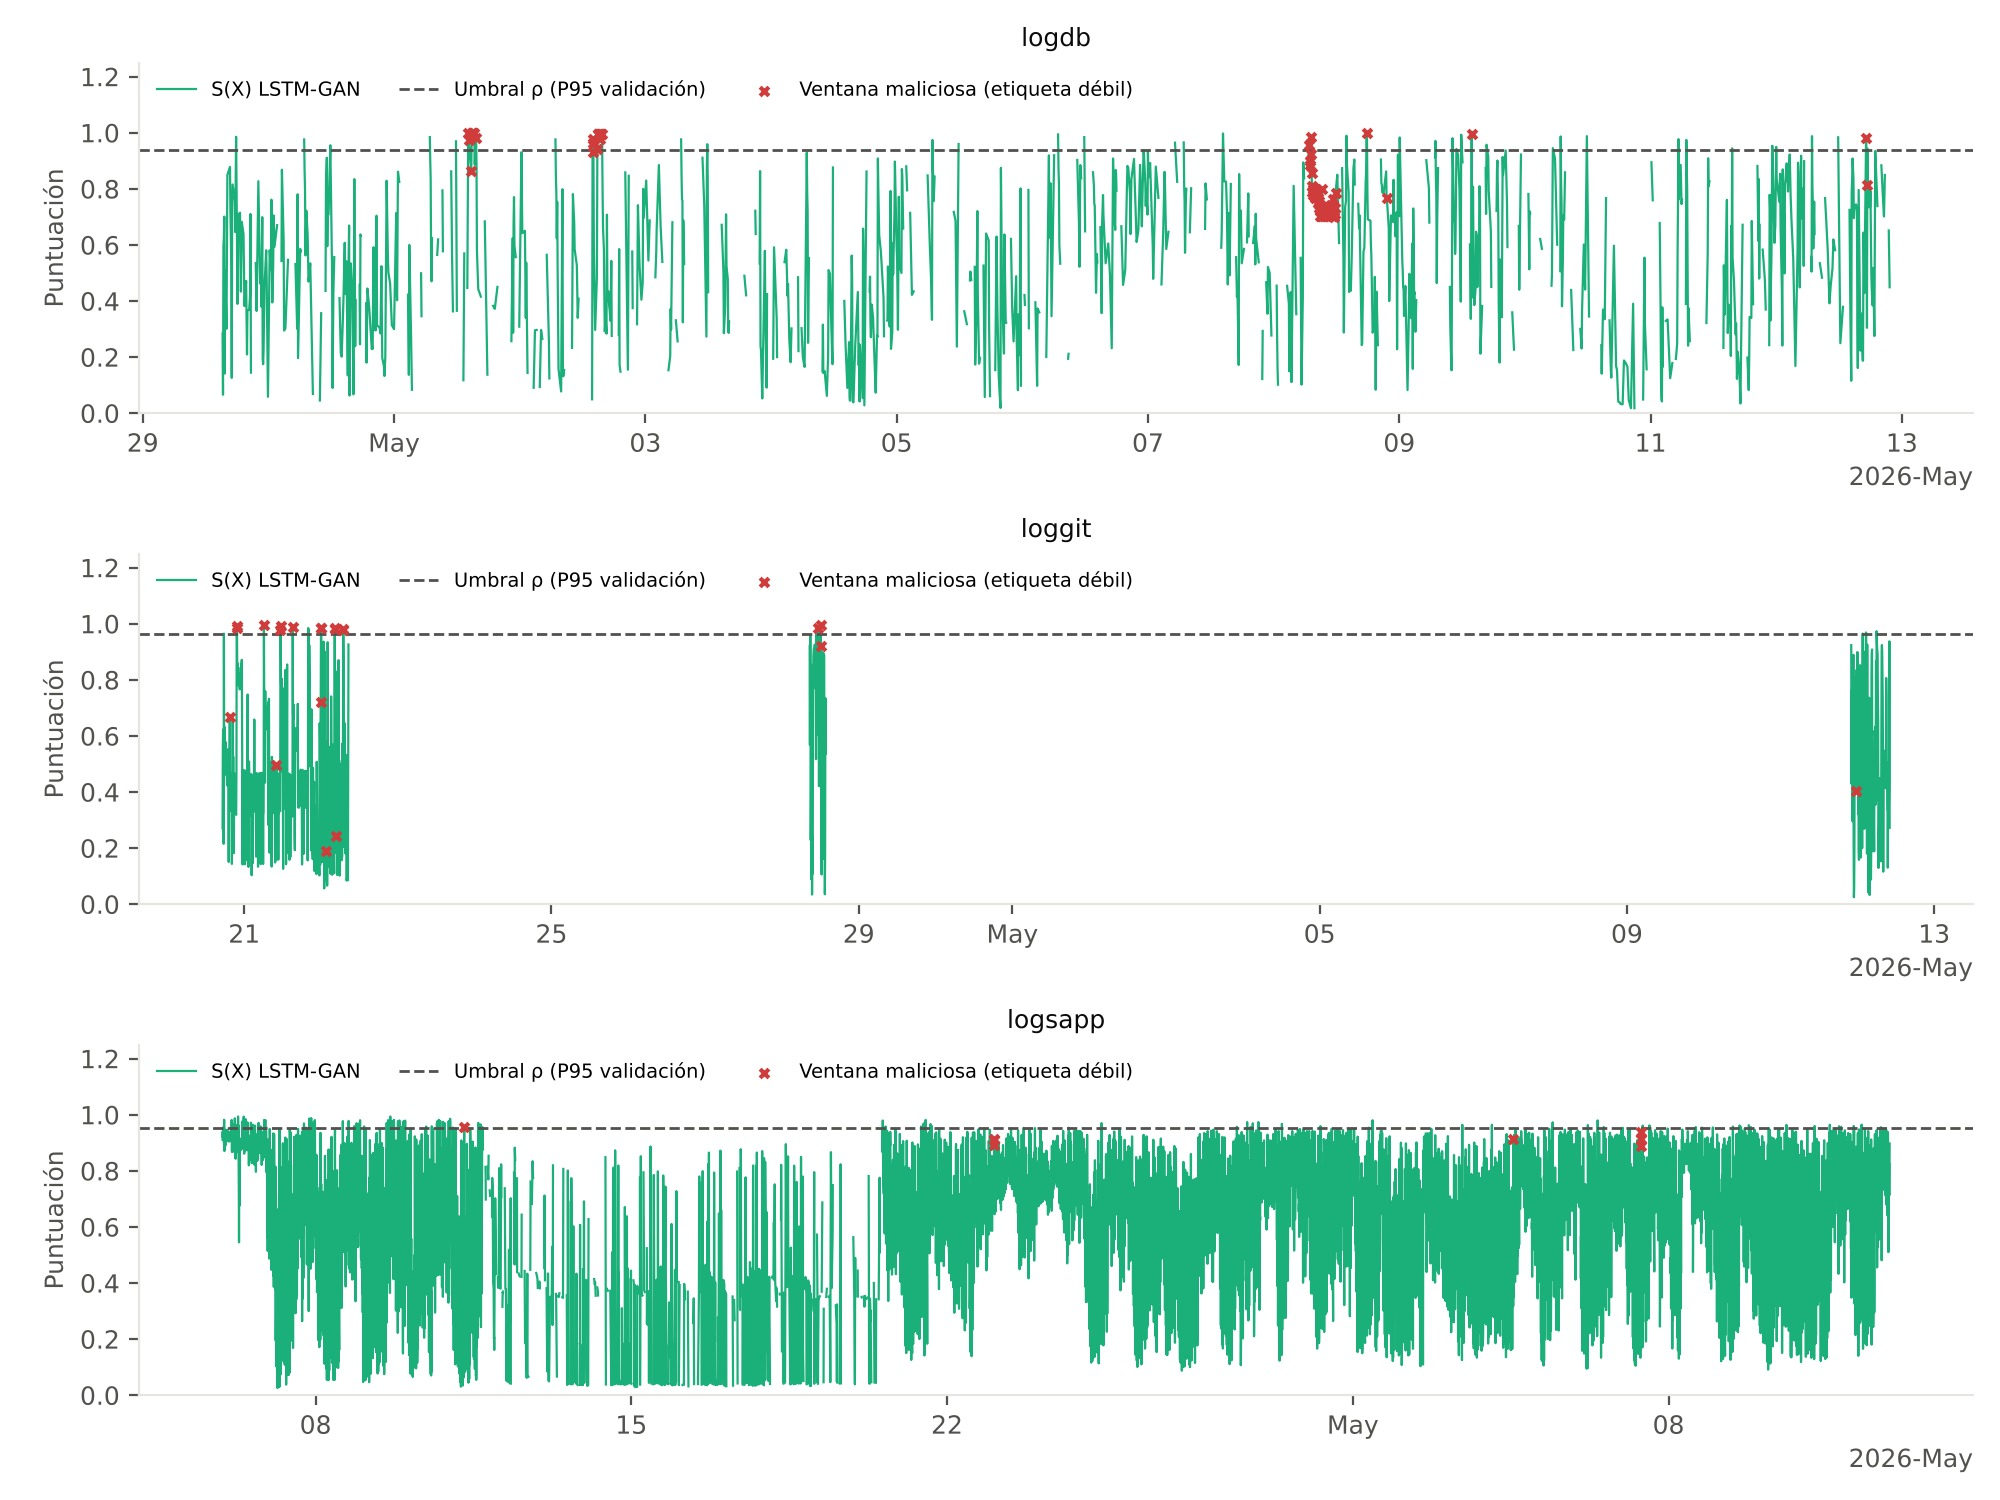
\includegraphics[width=\textwidth]{figs/fig3_serie_puntuacion.jpg}
\figurenote{Las cruces marcan ventanas con etiqueta débil maliciosa. Los huecos corresponden a periodos sin registros.}
\end{figure*}

% =====================================================================
\section{6. Discusión}
% =====================================================================
Los resultados respaldan parcialmente la hipótesis general. Coinciden con \textcite{gong2023} y \textcite{qian2025} en que la reconstrucción temporal de series latentes supera a los métodos estáticos en exactitud. La mejora observada, de 7.2 puntos de F1 y 54\,\% menos falsas alarmas, se explica porque Isolation Forest evalúa cada ventana de forma aislada, mientras que el LSTM interpreta el volumen y la composición de los eventos dentro de su contexto de 100 minutos. Esto es especialmente relevante en \texttt{logsapp}, cuyo tráfico de \textit{longpolling} varía a lo largo del día.

Sin embargo, a diferencia de \textcite{gong2023}, el componente adversarial no aportó valor sobre el autocodificador aislado e introdujo inestabilidad. Esto concuerda con las dificultades de entrenamiento de las GAN, como el desvanecimiento del gradiente y el colapso de modos, señaladas por \textcite{qian2025}. Una explicación plausible es que la contaminación del entrenamiento con ataques reales, ausente en los datos de sensores de esos estudios, lleva al discriminador a aprender también patrones maliciosos como reales.

La ventaja de Isolation Forest en el AUC de \texttt{loggit} confirma la advertencia de \textcite{landauer2023}: métodos simples pueden competir con el aprendizaje profundo cuando las anomalías se manifiestan como cambios de frecuencia, como ocurre con las ráfagas de escaneo web. Del mismo modo, los valores de F1 obtenidos, entre 1.9 y 62.6\,\%, son muy inferiores a los publicados sobre conjuntos de referencia, por ejemplo el 99.61\,\% de \textcite{nasirzadeh2025} o el 97.3\,\% de AUC de \textcite{gorokhov2023} en HDFS. Esta brecha es coherente con \textcite{albert2025}, quien mostró que la partición cronológica y la presencia de anomalías en el entrenamiento reducen drásticamente el desempeño reportado, y es comparable al F1 medio de 71.23\,\% de \textcite{zhao2025} en escenarios de transferencia entre sistemas.

En un contexto más amplio, el hallazgo de mayor valor operativo es la reducción de falsas alarmas sin etiquetas. En \texttt{logsapp} equivale a unas 840 alertas falsas menos durante el periodo de prueba de 30 días, lo que alivia directamente la carga de un equipo de seguridad universitario. La omisión de la enumeración lenta ilustra el límite de los modelos de contexto fijo ante anomalías colectivas de baja intensidad \parencite{zamanzadeh2024}. A ello se suma la sensibilidad al ruido de los registros reales, documentada por \textcite{zhang2025}.

\textbf{Limitaciones.} Las etiquetas débiles, derivadas de reglas, no equivalen a una verdad de campo y pueden omitir ataques no contemplados en ellas. Se analizaron tres de los cuatro subconjuntos del repositorio. \texttt{logsapp} cuenta con muy pocas ventanas maliciosas en el tramo de prueba. Por último, no se realizó una búsqueda de hiperparámetros para evitar ajustar el modelo sobre el tramo de evaluación.

\textbf{Líneas futuras.} Se proponen cinco:
\begin{enumerate}
  \item Calibrar $\rho$ según la tasa esperada de anomalías de cada servicio \parencite{qian2025}.
  \item Emplear contextos multiescala para capturar ataques lentos.
  \item Incorporar explicabilidad para el analista \parencite{landauer2023}.
  \item Transferir el modelo entre subsistemas mediante pseudoetiquetado \parencite{zhao2025}.
  \item Fusionar las modalidades semántica y secuencial con transformadores colaborativos \parencite{nasirzadeh2025}.
\end{enumerate}

% =====================================================================
\section{7. Conclusiones}
% =====================================================================
Se cumplió el propósito de evaluar el efecto del modelo de agentes adversarios duales LSTM--GAN sobre la detección de comportamientos maliciosos sin etiquetas en registros de servidores universitarios. Las hipótesis específicas se verificaron como sigue:

\begin{itemize}
  \item \textbf{H1 se valida.} El F1 aumentó de 25.06\,\% a 32.26\,\% ($p < .001$).
  \item \textbf{H2 se valida.} La FPR se redujo de 6.27\,\% a 2.88\,\% ($p = .002$).
  \item \textbf{H3 se rechaza.} El AUC no cambió de forma significativa ($p = .529$).
\end{itemize}

En consecuencia, la hipótesis general se acepta de forma parcial. La relevancia y novedad del estudio residen en evaluar este tipo de arquitectura sobre 3.2 millones de eventos crudos de tres servicios reales, con partición cronológica, entrenamiento contaminado y contraste estadístico. Se trata de condiciones más cercanas a la producción que las de los conjuntos de referencia habituales.

Los aportes principales son tres: una representación de ventanas como series semánticas que permite detectar ráfagas de ataque repetitivas, la evidencia mediante ablación de que la reconstrucción temporal y no el discriminador explica la mejora, y un repositorio reproducible. En cuanto a la aplicabilidad práctica, un equipo de seguridad universitario puede desplegar el modelo sin etiquetar datos y obtener menos de la mitad de falsas alarmas que con la técnica tradicional. Esto responde a la motivación inicial: aprovechar los abundantes registros institucionales sin depender de analistas para etiquetarlos.

% =====================================================================
\section*{Dataset y código fuente}
% =====================================================================
\begin{itemize}
  \item \textbf{Datos crudos:} subconjuntos \texttt{logdb}, \texttt{loggit} y \texttt{logsapp} del repositorio \textit{uni-logs} (\url{https://uni-logs.us-mia-1.linodeobjects.com/list.html}).
  \item \textbf{Código y resultados:} los guiones \texttt{prep.py}, \texttt{experiment.py} y \texttt{analyze.py}, el archivo \texttt{requirements.txt}, las tablas de resultados y las figuras están disponibles en \url{https://github.com/Arthur100803/ia2-tema7-agentes-adversarios-duales}.
  \item \textbf{Ejecución completa:} los comandos están en el archivo \texttt{README.md}. Toma unos 105 minutos en una CPU de dos núcleos.
\end{itemize}

% =====================================================================
\printbibliography
% =====================================================================

% =====================================================================
%  ANEXOS (una columna)
% =====================================================================
\onecolumn
\appendix
\section{Matriz de operacionalización de variables}

% >>> La rúbrica exige 2-4 dimensiones por variable y >= 2 indicadores por dimensión.
\begin{table}[h]
\caption{Matriz de operacionalización}
\label{tab:operacionalizacion}
\small
\begin{tabularx}{\textwidth}{@{}p{2.6cm}p{3.2cm}p{3.1cm}Xp{1.9cm}@{}}
\toprule
Variable & Dimensión & Indicador & Definición operacional / fórmula & Escala \\
\midrule
\multirow{6}{2.6cm}{\textbf{VI}: Modelo de agentes adversarios duales LSTM--GAN}
 & D1. Reconstrucción temporal & Error de reconstrucción ($\mathcal{L}_{rec}$) & Error cuadrático medio, ecuación~\eqref{eq:rec}, en validación & Razón \\
 & & Épocas hasta convergencia & Épocas hasta la parada temprana (paciencia 5) & Razón \\
 & D2. Discriminación adversarial & Pérdida del discriminador ($\mathcal{L}_D$) & Ecuación~\eqref{eq:ld} & Razón \\
 & & Probabilidad de rechazo & $1 - D(\tilde H_t)$ por ventana & Razón [0,1] \\
 & D3. Puntuación dual & Puntuación de anomalía $S_t$ & Ecuación~\eqref{eq:score} & Razón [0,1] \\
 & & Tasa de alerta & Proporción de ventanas con $S_t > \rho$ & Razón (\%) \\
\midrule
\multirow{6}{2.6cm}{\textbf{VD}: Detección de comportamientos maliciosos}
 & D1. Exactitud de la detección & Puntaje F1 & $2PR/(P+R)$ & Razón (\%) \\
 & & Precisión ($P$) y exhaustividad ($R$) & $TP/(TP+FP)$; $TP/(TP+FN)$ & Razón (\%) \\
 & D2. Tasa de falsas alarmas & Tasa de falsos positivos (FPR) & $FP/(FP+TN)$ & Razón (\%) \\
 & & Especificidad & $TN/(TN+FP) = 1 - \mathrm{FPR}$ & Razón (\%) \\
 & D3. Capacidad discriminante & Área bajo la curva ROC (AUC) & Área bajo la curva TPR--FPR & Razón (\%) \\
 & & Coeficiente de Matthews (MCC) & Correlación entre la clase real y la predicha & Intervalo [$-1$,1] \\
\bottomrule
\end{tabularx}
\figurenote{Instrumentos: guion \texttt{experiment.py} (VI) y matriz de confusión frente a las etiquetas débiles del Apéndice C (VD).}
\end{table}

\section{Matriz de consistencia}
\begin{table}[h]
\caption{Matriz de consistencia}
\label{tab:consistencia}
\scriptsize
\begin{tabularx}{\textwidth}{@{}XXXp{2.9cm}p{3.1cm}@{}}
\toprule
Problema & Objetivo & Hipótesis & Variables y dimensiones & Metodología \\
\midrule
\textbf{General:} ¿En qué medida el modelo LSTM--GAN mejora la detección de comportamientos maliciosos sin etiquetas en registros de servidores universitarios? &
\textbf{General:} Evaluar en qué medida el modelo LSTM--GAN mejora dicha detección frente a una técnica no supervisada tradicional. &
\textbf{General:} El modelo LSTM--GAN mejora significativamente la detección de comportamientos maliciosos. &
\textbf{VI:} Modelo LSTM--GAN (D1 reconstrucción temporal, D2 discriminación adversarial, D3 puntuación dual). &
\textbf{Enfoque:} cuantitativo. \textbf{Tipo:} aplicado. \textbf{Nivel:} explicativo. \textbf{Diseño:} cuasi-experimental pre-prueba/post-prueba con ablación. \\
\addlinespace
\textbf{PE1:} ¿En qué medida mejora la exactitud de la detección? &
\textbf{OE1:} Determinar el efecto sobre el puntaje F1. &
\textbf{H1:} El LSTM--GAN aumenta significativamente el F1. &
\textbf{VD:} Detección de comportamientos maliciosos (D1 exactitud). &
\textbf{Población:} eventos del repositorio \textit{uni-logs}. \textbf{Muestra:} 53\,416 ventanas de 5 min (3 subconjuntos), por conveniencia. \\
\addlinespace
\textbf{PE2:} ¿En qué medida reduce la tasa de falsas alarmas? &
\textbf{OE2:} Determinar el efecto sobre la FPR. &
\textbf{H2:} El LSTM--GAN reduce significativamente la FPR. &
(D2 tasa de falsas alarmas) &
\textbf{Técnica:} análisis documental. \textbf{Instrumentos:} Drain3, ficha de reglas (Apéndice C), guiones Python. \\
\addlinespace
\textbf{PE3:} ¿En qué medida mejora la capacidad discriminante? &
\textbf{OE3:} Determinar el efecto sobre el AUC-ROC. &
\textbf{H3:} El LSTM--GAN aumenta significativamente el AUC. &
(D3 capacidad discriminante) &
\textbf{Análisis:} estadística descriptiva; Wilcoxon pareado ($\alpha=.05$); \textit{bootstrap} del AUC. \\
\bottomrule
\end{tabularx}
\end{table}

\section{Instrumento de recolección de datos}
\textbf{C.1 Ficha de etiquetado débil por ventana.} Para cada ventana de cinco minutos se registran los campos \texttt{win} (inicio, UTC), \texttt{n\_events} (número de eventos), el conteo de cada regla de la Tabla~\ref{tab:reglas} (\texttt{sqli}, \texttt{probe}, \texttt{web}, \texttt{scan}, \texttt{ssh}, \texttt{c4xx}) y la etiqueta \texttt{y} $\in \{0,1\}$. El instrumento se aplica automáticamente con \texttt{prep.py} y su salida queda en los archivos \texttt{<subconjunto>\_windows.csv}.

\textbf{C.2 Ficha de registro de resultados por corrida.} Para cada combinación de subconjunto, semilla y modelo se registran los campos \texttt{epochs}, F1, precisión, exhaustividad, FPR, AUC, MCC, TP, FP, TN y FN. La salida queda en los archivos \texttt{results\_runs\_*.csv}.

\textbf{C.3 Validez y confiabilidad.} Las reglas se basan en indicadores de compromiso inequívocos en el contexto analizado: por ejemplo, las peticiones a \texttt{.php} carecen de uso legítimo en GitLab y en Odoo. La confiabilidad se garantiza porque el instrumento es determinista: la misma entrada produce siempre las mismas etiquetas.

\end{document}
